\section{Monotonicity and mean-field theory}
\label{sec:mf}

The model is attractive (monotone) when $w(j)$ is nondecreasing in $j$ and $w(j)+w(8-j)\le 1$,
because a site's probability of being alive after an update then increases with the set of live
sites. The second condition holds for $q\le(1-\alpha)(1-p)$.
The first requires both $(1-p)\alpha\le p/8$, from $j=3\to4$,
and $q\le(1-p)\alpha+p/8$, from $j=2\to3$.
Thus, at $\alpha=1/2$ and in the tested range
$q\le(1-p)/2$, the model is nonmonotone for $p<0.8$ and monotone
for $p\ge0.8$. These conditions do not cover the $\alpha=1$ checks.
None of our arguments uses monotonicity. Finite-time front and seed signatures
also occur in the monotone region; the strongest coexistence evidence below
is at the nonmonotone value $p=1/2$.
Monotone nonlinear voter models with two absorbing states and an
active phase in two dimensions are known, the threshold voter
models~\cite{liggett1994}; what is at issue here is the order of the transition, not the
existence of an active phase.

At the level of a pair approximation on the Bethe lattice with $z = 8$ (Supplemental Sec.~\ref{app:pa}),
the absorbing states are linearly stable for every $p<1$ and the disordered active state is
stable as well over the parameter range checked. The approximation is bistable
throughout that range and does not single
out a transition point: in a spatial system the phase is selected by which phase invades the
other. Mean-field bistability is precisely the situation in which washout is expected in two
dimensions~\cite{castellano2009}. Whether the two-dimensional transition is discontinuous is
therefore a question about fronts and fluctuations, and it is the question the simulations
address.

\section{Frozen configurations at $p = 0$}
\label{app:frozen}

At $p = 0$ the flip table is $w(j) = \alpha R(j) + q\,\delta_{j,2}$, so every configuration in
which all sites have $j\in\{0,1,4,5\}$ is frozen. A local construction proves
that their number grows exponentially with area. Start from a checkerboard
on a torus whose lengths are divisible by four. Independently choose whether
to complement each $2\times2$ block with lower-left corner $(4a,4b)$.
For one complemented block, its four sites and the four exterior diagonal
corners have $j=5$; the other sites in its surrounding $4\times4$ square
retain $j=4$. The affected neighborhoods of different blocks are disjoint,
so every choice is frozen. Hence, with $N=L_xL_y$,
\begin{equation}
 \mathcal N_{\rm frozen}\ge 2^{N/16},\qquad
 \frac{\ln\mathcal N_{\rm frozen}}{N}\ge\frac{\ln2}{16}.
 \label{eq:frozenbound}
\end{equation}
This bound holds for every admissible $q$ at $p=0$.

Transfer-matrix counts on periodic strips of fixed widths $W=7$ and $8$
give a larger strip entropy, $\mathcal N_W\sim e^{s_WN}$ with
$s_W\approx0.32$ per site, against $\ln2\simeq0.69$ for all configurations.
These two strip widths do not determine the two-dimensional entropy density.
As a check,
on the $3\times3$ torus, where every site neighbors every other, the count is
$254 = 1 + \binom94 + \binom95 + 1$. The simplest examples are the two checkerboards and the
diagonal stripes of width two, in which every site has $j = 4$.

These exceptional configurations did not attract the tested random starts at $q>0$. Random initial conditions at $L = 256$
run to $t = 10^6$ at $q = 0.005$--$0.018$ (all below $\qs$) end in one of the two uniform states.
In the active phase ($q = 0.03$--$1$) the frequency of locally checkerboard or stripe-like
$3\times3$ blocks stays at the level expected by chance. A prepared half-lattice of either pattern
next to an active or a dead half is eroded completely within $10^4$ steps at every $q$ tested,
including $q = 0$, and a single flipped site destroys a perfect $256\times256$ pattern within
$\approx 10^3$ steps (in 11 of 12 runs). Only at $q = 0$, where $j = 2$ sites are also frozen, does
the dynamics stop with a small density ($\approx 1\%$) of frozen debris.

Removing the frozen configurations directly by a flip probability $\epsilon$ at
$j\in\{1,4,5\}$ preserves the linear reversal of the front velocity: at $\epsilon = 0.003$ the
velocity is $-0.0041$, $-0.0002$, $+0.0024$, $+0.0053$ at $q/\qs(0) = 0.88$, 0.92, 0.96, 1.00, so
$\qs(\epsilon)\approx 0.92\,\qs(0)$, and at $\epsilon = 0.01$, $\qs\approx 0.8\,\qs(0)$, with
an interior interface fraction 0.44--0.6 behind the front. These checks retain
front reversal and an active interior after removing the extra frozen states.
They suggest a smooth small-$\epsilon$ continuation over the measured range;
they do not establish the infinite-time $p\to0^+$ limit of the voter-admixed family.

\section{Pair approximation}
\label{app:pa}

We closed the dynamics at the level of nearest-neighbor pairs on a Bethe lattice with $z = 8$:
given a site's state, its neighbors are independent and disagree with it with probability
$\theta_s = \rho/(2x_s)$, where $\rho$ is the fraction of disagreeing bonds and $x_s$ the fraction
of sites in state $s$. Both the continuous-time version and the synchronous map were analyzed.
In the voter limit the continuous-time closure conserves $m$ and gives $\rho^*=(z-2)(1-m^2)/[2(z-1)]$. The synchronous map differs: at $m=0$ its active fixed point is $\rho^*=1/2$. For every
$p<1$ a dilute minority in an absorbing state decays at rate
$(1-p)\alpha P_R(\theta) + qP_2(\theta)$, where $\theta$ is the conditional
disagreement probability around a minority site,
$P_j(\theta)=\binom{8}{j}\theta^j(1-\theta)^{8-j}$, and
$P_R=P_3+P_6+P_7+P_8$. Thus the absorbing states are linearly stable in the
parameter range studied, and the
symmetric active fixed point ($\rho^*\approx 0.43$--$0.50$) is stable over the
parameter grid checked. The approximation is bistable over that grid and
does not select a coexistence point; a
front criterion based on it gets $\qs\propto(1-p)$ near the voter point but with an amplitude off
by a factor of two, and fails qualitatively for $p\lesssim 0.5$. This motivates the finite-time closure examined in Sec.~\ref{M-sec:theory}.

\section{A second rule: noise on the forbidden flips of D\&N}
\label{app:eta}

To check that the discontinuity does not depend on the voter admixture, we studied the rule
\begin{equation}
w(j) = \alpha R(j) + \eta\,[\,j\in\{1,2,4,5\}\,],
\label{eq:eta}
\end{equation}
in which every flip that D\&N forbids, except at $j = 0$, happens with a small probability $\eta$.
For $0<\alpha,\eta\le1$, the lemma of Sec.~\ref{M-sec:lemma} gives exactly
two absorbing states. At $\alpha = 1/2$, strip
fronts ($L_x = 2048$, $L_y = 4096$, $T = 10^5$, three seeds) retreat at $v = -0.0022\pm0.0010$ for
$\eta = 0.01275$ and advance at $v = +0.0020\pm0.0001$ and $+0.0054\pm0.0001$ for $\eta = 0.013125$
and $0.01375$, so $\eta^*\approx 0.0130$ (linear interpolation: $0.01295$). Bulk runs at $L = 1024$ and 2048 (two seeds each,
$T = 2\times10^5$) have last-half interface densities
$\rho\simeq0.25$ at $\eta = 0.013125$ ($\approx
1.01\,\eta^*$) and $\rho\simeq0.276$ at $0.01375$, at both sizes. Below $\eta^*$ the prepared active phase decays: at $\eta = 0.01275$ it decays slowly (from $\rho = 0.236$ at $t = 10^4$ to $0.17$ at
$2\times10^5$), and at $\eta = 0.0125$, $0.01225$, $0.011875$, and $0.01125$ its half-life is
$(5.3$--$6.4)\times10^4$, $(2.6$--$3.2)\times10^4$, $(1.3$--$1.6)\times10^4$, and $(0.8$--$0.9)
\times10^4$, similar at the two sampled sizes. Here the half-life is the first
recorded crossing below half the density at $t=10^3$, rather than consensus.
Together these finite-window front and bulk checks support a discontinuity
with an active-side density of order 0.25 in this second rule
(Fig.~\ref{fig:eta}).

\begin{figure}
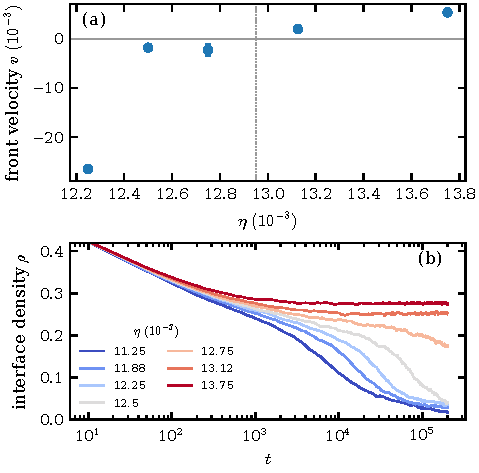
\includegraphics[width=\columnwidth]{figs/fig_eta}
\caption{The rule of Eq.~\eqref{eq:eta} at $\alpha = 1/2$. (a) Strip-front velocity against $\eta$
(three runs per $\eta$; plotted means retain fits with at least 20 records,
including only two runs at $\eta=0.01225$). The strongly negative
$\eta=0.01225$ estimate uses a short window before the strip interior orders;
it is not a late planar-front velocity. The dotted line is
$\eta^*=0.01295$. (b) Example bulk trajectories (seed 1) at $L=2048$.}
\label{fig:eta}
\end{figure}

